\documentclass[10pt]{article}
\usepackage{pgfplots}
\pgfplotsset{compat=1.16}

\begin{document}

\begin{figure}[h]
    \centering
    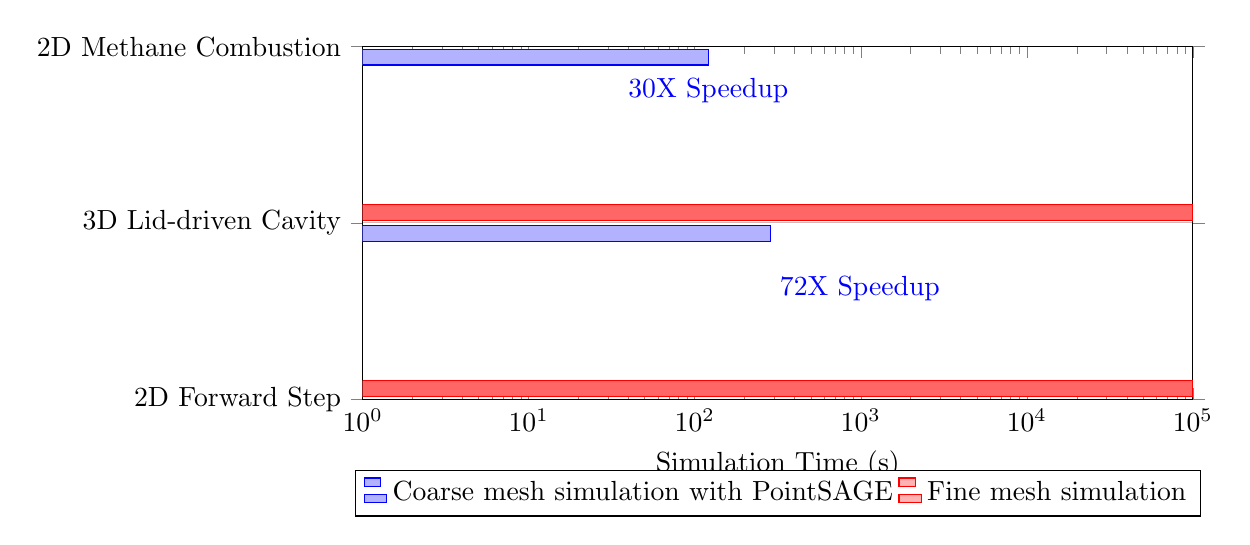
\begin{tikzpicture}
        \begin{axis}[
            width=\columnwidth,
            height=0.5\columnwidth,
            xlabel={Simulation Time (s)},
            xmode=log,
            xmin=1, xmax=100000,
            ymin=0, ymax=2,
            ytick={0,...,2},
            yticklabels={{2D Forward Step},{3D Lid-driven Cavity},{2D Methane Combustion}},
            legend style={at={(0.5,-0.2)},anchor=north,legend columns=-1},
            nodes near coords,
            point meta=explicit symbolic,
            xbar,
            bar width=0.2cm,
            visualization depends on=y \as \ymark,
            every node near coord/.append style={
                anchor=\ymark*90+90, yshift=-0.7cm
            },
            ymajorgrids=true
        ]
            \addplot coordinates {
                (84.8,0) [92X Speedup] % 2D Methane Combustion
                (284.6,1) [72X Speedup] % 3D Lid-driven Cavity
                (120.8,2) [30X Speedup] % 2D Forward Step
            };
            \addplot coordinates {
                (99999.9,0)
                (99999.9,1)
                (99999.9,2)
            } [fill=red!60];
            \legend{Coarse mesh simulation with PointSAGE, Fine mesh simulation};
        \end{axis}
    \end{tikzpicture}
    \caption{Comparison of Speedup Achieved by PointSAGE in Accelerated CFD Simulations. The blue bars represent the time taken for coarse mesh simulation along with the inference time of PointSAGE for predicting fine mesh simulation, while the red bars represent the simulation time for fine mesh simulation using the CFD solver OpenFOAM.}
    \label{fig:speedup_comparison}
\end{figure}

\end{document}